% !TeX spellcheck = cs_CZ
{\tikzset{external/prefix={tikz/FYZII/}}
 \tikzset{external/figure name/.add={ch11_}{}}
%---------------------------------------------------------------------------------------------------
% file fey2ch11.tex
%---------------------------------------------------------------------------------------------------
%=========================== Kapitola: Vnitřní stavba dielektrik ===================================
\chapter{Vnitřní stavba dielektrik}\label{fyz:IIchaXI}
\minitoc
  \section{Molekulové dipóly}\label{fyz:IIchaXIsecI}
  \section{Elektronová polarizace}\label{fyz:IIchaXIsecII}
  \section{Polární molekuly. Orientační polarizace}\label{fyz:IIchaXIsecIII}
  \section{Elektrické pole v dutinách dielektrika}\label{fyz:IIchaXIsecIV}
  \section{Permitivita kapalin. Clausiova-Mosottiova rovnice}\label{fyz:IIchaXIsecV}
  \section{Pevná dielektrika}\label{fyz:IIchaXIsecVI}
  \section{Feroelektřina. BaTiO3}\label{fyz:IIchaXIsecVII}
  \section{Příklady a cvičení}\label{fyz:IIchaXIsecVIII}

    \begin{figure}[ht!]
      \centering
      \begin{tabular}{c}
        \subfloat[ ]{\label{fyz_fig714a}
          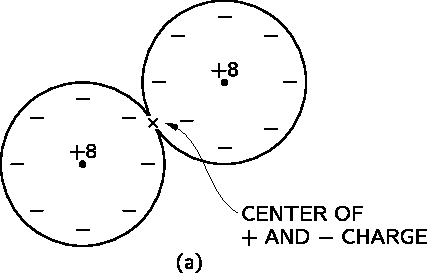
\includegraphics[width=0.6\linewidth]{fyz_fig714a.pdf}}               \\
        \subfloat[ ]{\label{fyz_fig714b}
          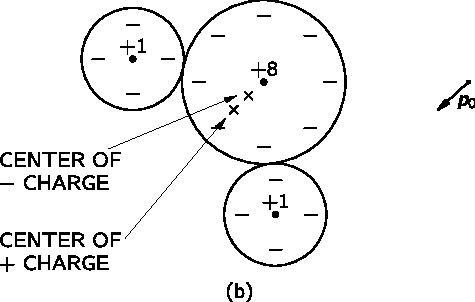
\includegraphics[width=0.6\linewidth]{fyz_fig714b.pdf}}
      \end{tabular}
      \label{fyz_fig714}
      \caption{
               (\cite[s.~748]{Feynman02})}
    \end{figure}

    \begin{figure}[ht!]
      \centering
      \begin{tabular}{c}
        \subfloat[ ]{\label{fyz_fig715a}
          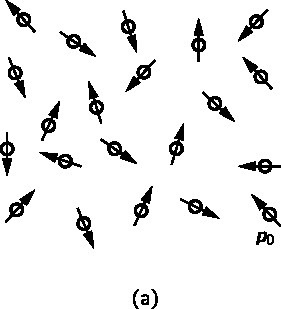
\includegraphics[width=0.6\linewidth]{fyz_fig715a.pdf}}               \\
        \subfloat[ ]{\label{fyz_fig715b}
          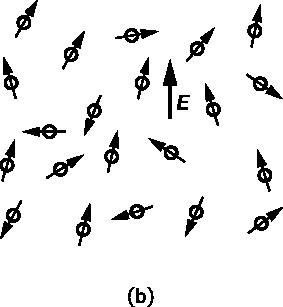
\includegraphics[width=0.6\linewidth]{fyz_fig715b.pdf}}
      \end{tabular}
      \label{fyz_fig715}
      \caption{
               (\cite[s.~748]{Feynman02})}
    \end{figure}

    \begin{figure}[ht!] %\ref{fyz_fig716}
      \centering
      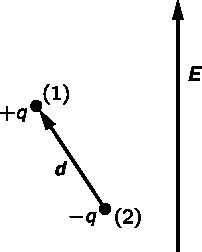
\includegraphics[width=0.7\linewidth]{fyz_fig716.pdf}
      \caption{
               (\cite[s.~707]{Feynman02})}
      \label{fyz_fig716}
    \end{figure}

    \begin{figure}[ht!] %\ref{fyz_fig717}
      \centering
      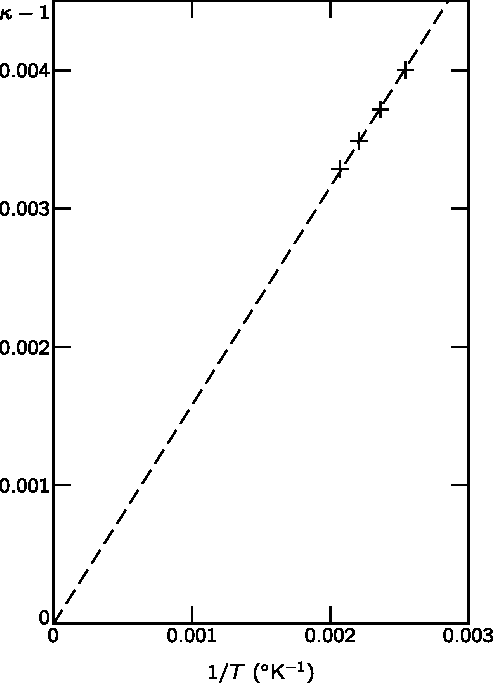
\includegraphics[width=0.7\linewidth]{fyz_fig717.pdf}
      \caption{
               (\cite[s.~707]{Feynman02})}
      \label{fyz_fig717}
    \end{figure}

    \begin{figure}[ht!] %\ref{fyz_fig718}
      \centering
      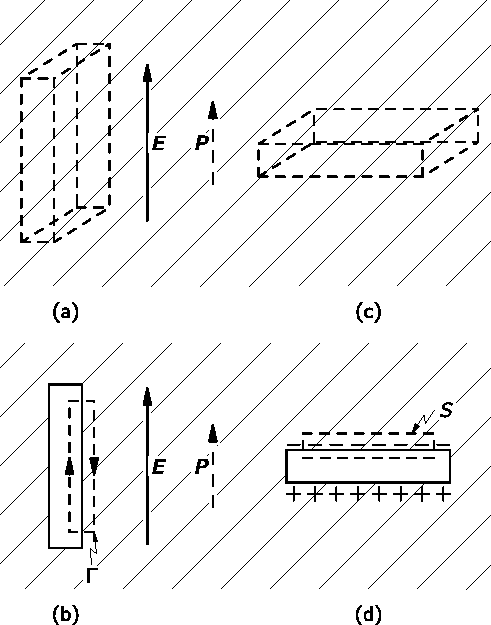
\includegraphics[width=0.7\linewidth]{fyz_fig718.pdf}
      \caption{
               (\cite[s.~707]{Feynman02})}
      \label{fyz_fig718}
    \end{figure}

    \begin{figure}[ht!] %\ref{fyz_fig719}
      \centering
      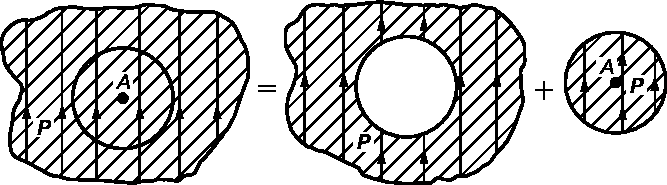
\includegraphics[width=0.7\linewidth]{fyz_fig719.pdf}
      \caption{
               (\cite[s.~707]{Feynman02})}
      \label{fyz_fig719}
    \end{figure}

    \begin{figure}[ht!] %\ref{fyz_fig720}
      \centering
      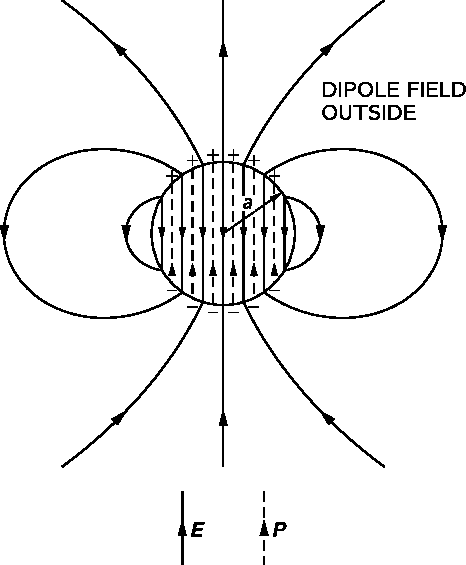
\includegraphics[width=0.7\linewidth]{fyz_fig720.pdf}
      \caption{
               (\cite[s.~707]{Feynman02})}
      \label{fyz_fig720}
    \end{figure}

    \begin{figure}[ht!] %\ref{fyz_fig721}
      \centering
      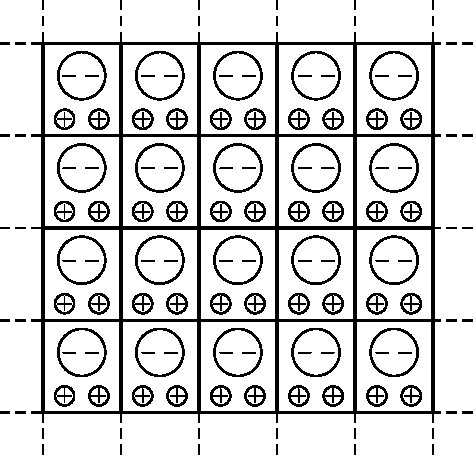
\includegraphics[width=0.7\linewidth]{fyz_fig721.pdf}
      \caption{
               (\cite[s.~707]{Feynman02})}
      \label{fyz_fig721}
    \end{figure}

    \begin{figure}[ht!] %\ref{fyz_fig722}
      \centering
      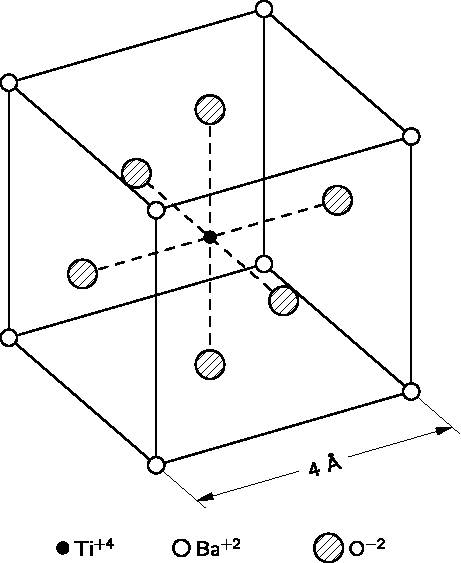
\includegraphics[width=0.7\linewidth]{fyz_fig722.pdf}
      \caption{
               (\cite[s.~707]{Feynman02})}
      \label{fyz_fig722}
    \end{figure}

    \begin{figure}[ht!] %\ref{fyz_fig723}
      \centering
      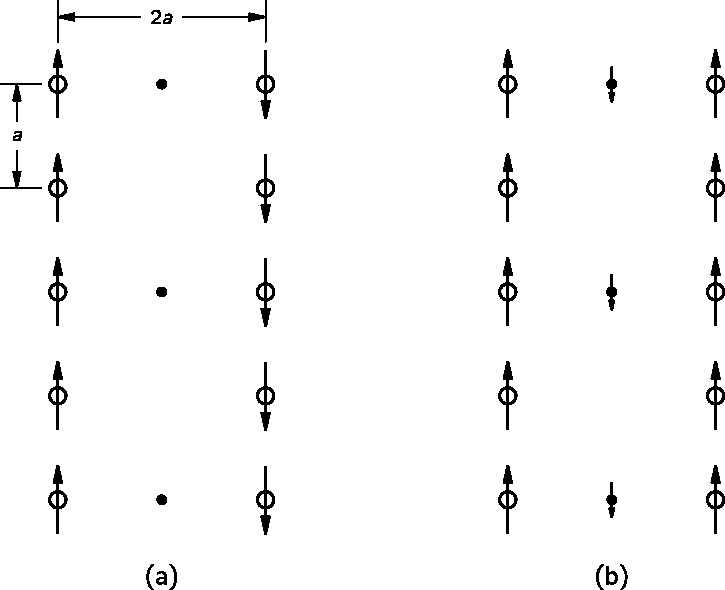
\includegraphics[width=0.7\linewidth]{fyz_fig723.pdf}
      \caption{
               (\cite[s.~707]{Feynman02})}
      \label{fyz_fig723}
    \end{figure}


} %tikzset
%---------------------------------------------------------------------------------------------------
%\printbibliography[title={Seznam literatury},heading=subbibliography]
\addcontentsline{toc}{section}{Seznam literatury}